\documentclass[a4paper, 10pt]{article}
\usepackage{graphicx}
\usepackage{amsmath}
\usepackage{amssymb}
\usepackage{listings}
\usepackage{appendix}
\usepackage{natbib} \setlength{\bibsep}{4.0pt}
\usepackage{bm}
\usepackage{subfig}
\usepackage{enumitem}
\usepackage{url}
\usepackage{array}
\usepackage{arydshln}
\usepackage{changepage}
\usepackage{url}
\usepackage{color}
\usepackage{lipsum}
\usepackage[percent]{overpic}


\newcommand{\exedout}{%
  \rule{0.8\textwidth}{0.5\textwidth}%
}

\addtolength{\oddsidemargin}{-.875in}
	\addtolength{\evensidemargin}{-.875in}
	\addtolength{\textwidth}{1.75in}

	\addtolength{\topmargin}{-.875in}
	\addtolength{\textheight}{1.75in}
	
% wide page for side by side figures, tables, etc
\newlength{\offsetpage}
\setlength{\offsetpage}{1.0cm}
\newenvironment{widepage}{\begin{adjustwidth}{-\offsetpage}{-\offsetpage}%
    \addtolength{\textwidth}{2\offsetpage}}%
{\end{adjustwidth}}


\begin{document}
\title{Selection efficiencies in signal only sample for $p \rightarrow \mu^{+} \gamma$ and $p \rightarrow e^{+} \pi^{0}$ nucleon decay modes in MicroBooNE}
\author{William De Rocco, Elena Gramellini}

\maketitle

\begin{abstract}
The study of nucleon decay in liquid argon time projection chambers (LArTPCs) is a subject of much interest since it widens nucleon decay searches to modes hardly detectable with other technologies. Assessing the performances of LArTPCs  for complex topologies detection and background rejection is crucial for future massive LArTPCs like DUNE~\cite{Adams:2013qkq}.\\
This note is the first of a series of 3 tech notes and addresses the first step towards assessing background processes to nucleon decay in MicroBooNE. Specifically, a procedure for the identification of the $p \rightarrow \mu^{+} \gamma$ and $p \rightarrow e^{+} \pi^{0}$  decay modes in MicroBooNE is presented along with preliminary selection efficiencies. Since the reconstruction of 3D objects plays a fundamental role in the identification of the nucleon decay modes, track reconstruction has been optimized for the $p \rightarrow \mu^{+} \gamma$ mode. The study of cosmogenic background will be addressed in a future note.

\end{abstract}

\tableofcontents
\newpage

\section{Introduction}

In the Standard Model, baryon number is conserved, causing for the proton and bounded neutrons to be stable. However, many Grand Unified Theories (GUTs) predict the nucleon decay on long time-scales. Both gauge-mediated GUTs, in which new gauge bosons are introduced that allow for the transformation of quarks into leptons and vice versa, as well as supersymmetric GUTs allow for the nucleon decay. The experimental identification of even one proton decay would point to an indirect proof of GUTs and is therefore a subject of great interest~\cite{Adams:2013qkq}.

Previous experiments have placed limits on the proton lifetime ~\cite{Akiri:2011dv}. The dominant experimental setup for these searches as historically been a water Cherenkov detector. This technology suffers from an inability to reconstruct  events  thru decay products that are below the Cherenkov threshold and relays on the gammas from nuclear deexcitation for those modes.

For this reason, an attractive alternate approach to identifying proton decay is the use of a liquid argon time projection chamber (LArTPC). LArTPCs have the ability to identify nucleon decay modes that a water Cherenkov detector has less sensitivity to, most notably the $p\rightarrow K^{+} \bar{\nu}$.  Previous MC studies ~\cite{Bueno:2007um} have claimed a very high selection efficiency of many nucleon decay topologies, making this an important area of study.

Future LArTPC experiments such as DUNE (Deep Underground Neutrino Experiment) will have active volumes large enough and will run for lengths of time that would allow for the identification of nucleon decay in liquid argon or, alternatively in the case of a null result, the ability to bound the proton lifetime in many channels. Though the active volume of MicroBooNE is too small to be able to place any limits on nucleon decay lifetimes, it provides an excellent source of data on backgrounds, primarily from cosmogenic sources, that will affect future proton decay searches in LArTPCs.
Previous work has been done to assess the potential identification efficiencies for different decay modes in a LArTPC ~\cite{Bueno:2007um} but as of yet, no study of selection efficiencies and dominant backgrounds to proton decay in LArTPCs has been performed with data, nor taking into account reconstruction efficiencies. This note discusses the first step of an analysis that will make the first investigation into proton decay backgrounds in MicroBooNE.


\section{Strategy}
The general strategy to identify nucleon decay backgrounds in MicroBooNE consist in the following 5 steps: 
\begin{enumerate}[topsep=10pt,itemsep=-1ex,partopsep=10pt,parsep=1ex]
\item Study the signal in MC
\item Fixing selections and workflow in MC, calculate the selection efficiency
\item Apply analysis framework to cosmics MC 
\item Apply analysis framework to cosmics data
\item Count how many cosmics events pass our selections.
\end{enumerate}

This note concerns exclusively step number 3 for the $p \rightarrow \mu^{+} \gamma$ and $e^{+} \pi^{0}$  decay modes. \\
Steps number 1 and 2, fundamental for what follows,  are described in MY FIRST TECHNOTE. 
We apply the same outflow as described in in MY FIRST TECHNOTE on comics MC set. The rejection power of our cutflow is defined as the ratio between the number of candidates post-cut flow and the number of candidates pre-cut flow.

\section{MC samples}
 We utilized mcc6.1 cosmics  sample for each mode. This sample was generated using larsoft and uboonecode version v04\_12\_00, CRY cosmics generator, standard reconstruction. The events were converted to larlite format. We analyzed  NEEDS TO BE CHANGED events. \\
We used the reco data products "showerrecopandora" for shower reconstruction and "kalmanhit" for track reconstruction. Additional studies with different data products are viable, but not  yet performed.\\


\section{$p \rightarrow \mu^{+} \gamma$}
The following paragraphs address the analysis of the  $p \rightarrow \mu^{+} \gamma$  proton decay mode. This mode is particularly interesting for background searches in MicroBooNE: given MicroBooNE surface positioning, we expect an important statistical background.
The signal topology for this mode is constituted by one electromagnetic shower and one track pointing back to a common origin.

%The aim of what follows is to describe a set of cuts designed to isolate this signal from background, and to further discuss the types of cosmogenic background events that can fake this signal.

\subsection{Signal only analysis}

In an attempt to isolate this signal, the following procedure was implemented (for a detailed explanation about running the code, see Appendix A ):
\begin{enumerate}[topsep=10pt,itemsep=-1ex,partopsep=10pt,parsep=1ex]
\item Tracks refinements
\item Passing thru tracks cuts and loose energy cuts
\item Combinatorics pairing 
\item Geometrical cuts
\item PID and Calorimetry cuts 
\end{enumerate}

\subsubsection{Tracks refinement}
\label{trackRef}
Hand scanning reconstructed events and comparing the  length of MCReco tracks with the length of Reco tracks highlighted some pathologies of track reconstruction. The following three aspects were particularly noticeable:
\begin{enumerate}[topsep=10pt,itemsep=-1ex,partopsep=10pt,parsep=1ex]
\item there are cases where the gamma shower is reconstructed as one or multiple tracks
\item there are cases where the michel electron is attached to the muon track
\item there are cases where the gamma is attached to the muon track
\end{enumerate}


As a first action to eliminate the mis-reconstructed showers from the track pool, only tracks with more than 10 3D points in MCReco data product and tracks with more than 100 3D points in Reco data product are selected\footnote{The difference in the value of this cut is due to the way the MCReco and Reco data products are stored. The MCReco track data product saves only the 3D points where physics process takes place in G4. On the contrary, the spacing among 3D points in Reco track data products is driven by actual wire separation (3mm), and therefore a count of trajectory points is inherently different from MCReco track data product.}. In general, showers reconstructed as tracks have very only a few 3D points.  \\
Then, we apply a technique to refine the edges of the track. We start assuming that the central part of the track is well reconstructed and that the 3D mis-association can occur only at the edges. We divide the track in 5 segments, each containing a fifth of the total number of 3D points. We analyze the first and last segment. In the first segment, we calculate the distance between each 3D point starting from the first 3D point. If the distance is greater that 5 cm for Reco tracks (100 cm for MCReco), we claim the existence of a ``gap". All the points before the gap are removed from the track. The same procedure is performed on the last segment of the track, starting from the last 3D point. We define then the edges of the refined track to be the first point of after the gap in the first segment and the first point before the gap in the last segment. We are using here the concept of track edge instead of beginning and end of the track since the track direction is not defined. In order to calculate the energy deposited by the track, we multiply the length of the refined track by 2.3 MeV/cm. No Bragg peak correction is performed.



\subsubsection{Combinatoric pairing}
As the first stage of event selection, we perform a combinatoric pairing. Every combination of one shower and one track is kept as a preliminary candidate. This implies that the muon track can be paired to its michel electron at times. The idea of this stage is to be as inclusive as possible, even at the risk of over-identify pairs in the event. Further cuts are applied at a later stage will eliminate mis-id pairs, like muon - michel e pairs.

\subsubsection{Passing thru tracks cuts and loose energy cuts}
The second stage of event selection is the application of some  loose cuts. Every track passing thru the detector is discarded.
The track is defined as ``passing thru"  if one of the following conditions is met:
\begin{enumerate}[topsep=10pt,itemsep=-1ex,partopsep=10pt,parsep=1ex]
\item edge 1 x $>$ 3 cm       and  edge 2  x $<$  250 cm
\item edge 1 y $>$ -113 cm and  edge 2 y $<$ 113 cm
\item edge 1 z $>$ 3 cm       and  edge 2 z $<$ 1050 cm
\end{enumerate}
It is important to notice that this selection keeps tracks that originates in the detector but are not contained and tracks that enter and stop the detector. 
Shower and tracks with energy deposition greater than 2 GeV are also discarded. 
%\begin{figure}[h!]
%\centering
%\begin{minipage}{0.45\textwidth}
%\centering
%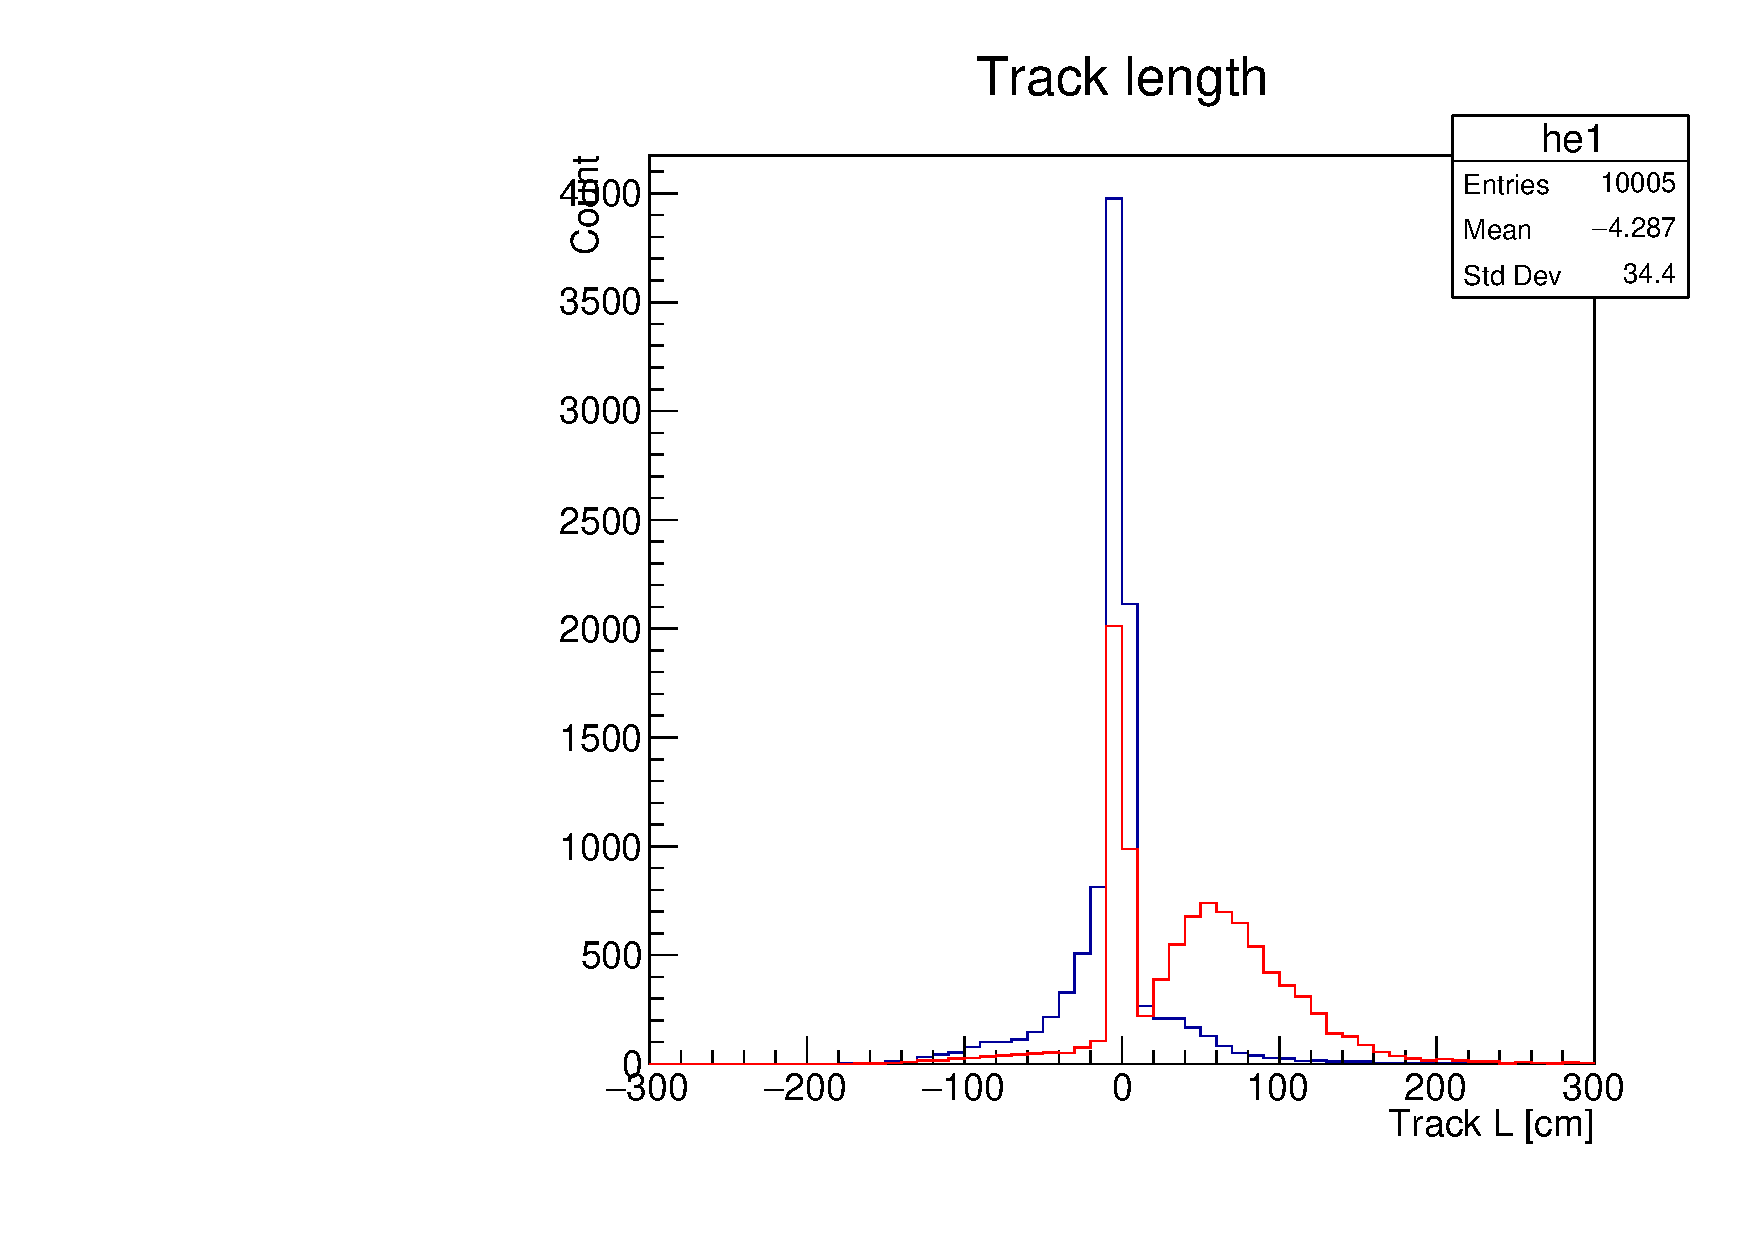
\includegraphics[width=3in]{DiffLeng.pdf}
%\caption{Difference in length, Reco -  MCReco.  The refined length with $\Delta$ = 5 cm is plotted in blue, the length from data product is plotted in red.\\}
%\end{minipage}\hfill
%\begin{minipage}{0.45\textwidth}
%\centering
%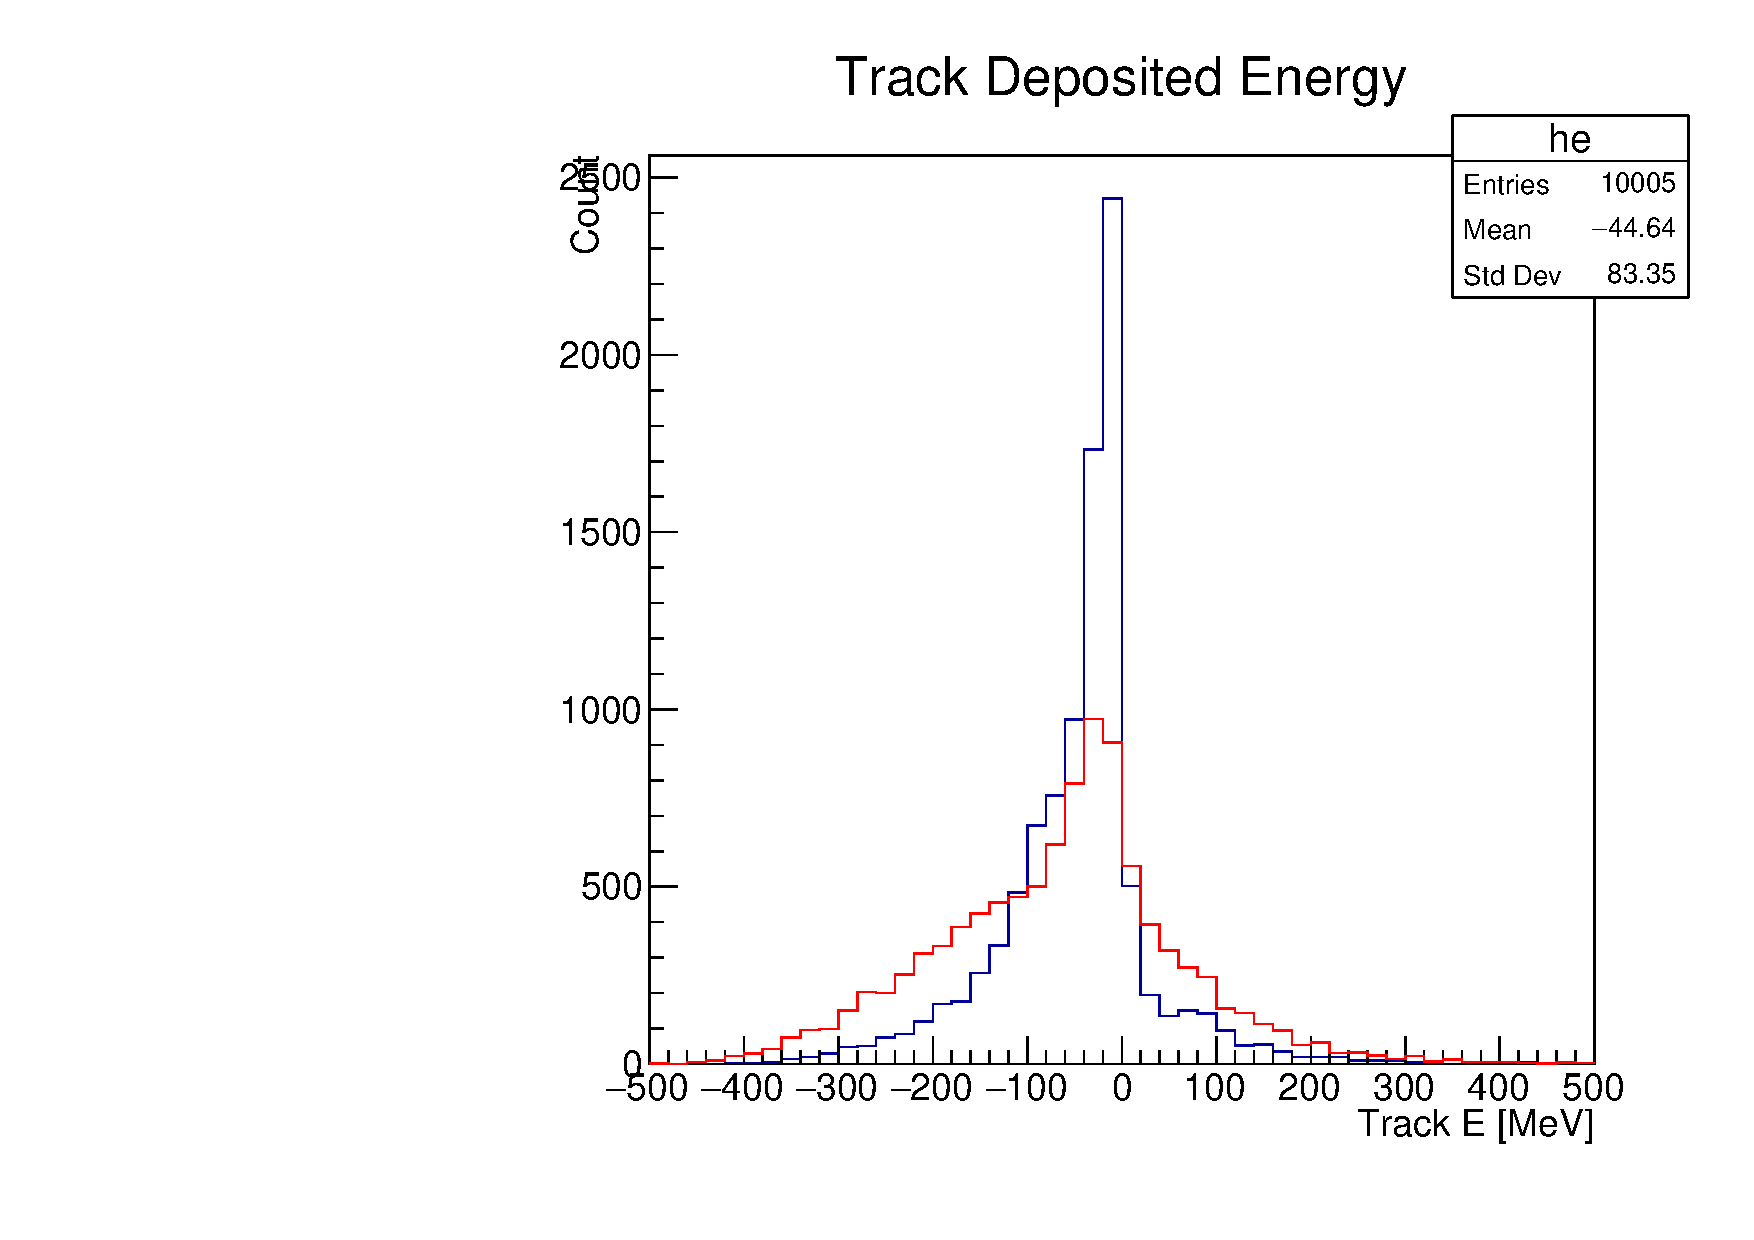
\includegraphics[width=3in]{DiffEn.pdf}
%\caption{Difference in energy, Reco - MC Reco. In blue, the energy is obtained  multiplying  the refined length by mip dEdx, no bragg peak correction. In red ,energy deposition from data product.}
%\end{minipage}
%\end{figure}


%\begin{figure}[h!]
%\begin{center}
%\begin{overpic}[width=6in]{LengthCutStudy.pdf}
%\put (17,85) {$\displaystyle\Delta = 20$ cm}
%\put (17,55) {$\displaystyle\Delta= 5$ cm}
%\put (17,20) {$\displaystyle\Delta= 1$ cm}
%\put (60,85) {$\displaystyle\Delta= 10$ cm}
%\put (60,55) {$\displaystyle\Delta= 2$ cm}
%\end{overpic}
%\caption{Track length (blue) MC Reco and (red) refined reco for different $\Delta$. }
%\end{center}
%\end{figure}


\subsubsection{Geometrical cuts}
Three geometrical cuts are then applied.  
The first geometrical cut performed is a cut on the angle between the 3-momenta of the reconstructed $\mu$ and $\gamma$. Naively, this would be expected to be steeply peaked near $\pi$ because the proton decays at rest and momentum is conserved. This is not the case. Two factors contribute to this. The first is that the proton does not decay at rest, but instead decays with some momentum less than the Fermi momentum of the nucleus, which is on the order of 200 MeV/$c$.  In addition to this effect, the direction of the track is mis-reconstructed at times. This implies the opening angle distribution to be peaked at both 0 and $\pi$. For these reasons, the opening angle cut is quite loose, since we keep pairs with angle greater than 1.2 rad and pairs with angle less than 0.5 rad.\\
The second geometrical cut is a cut on the distance of closest approach between the shower and the track (the impact parameter, IP). This cut assesses the coplanarity of shower and track. The third geometrical cut is a cut on the distance between the start point of the shower and the start point of the track. We define the ``start point of the track" to be the track edge closest to the shower under consideration. This cut serves as a proximity cut. 


\subsubsection{PID and Calorimetry cuts }
\label{ID}
After geometrical cuts are performed, PID and calorimetric cuts on the decay products and reconstructed proton are performed. Only muons and pions are kept, the PID information being retrieved from the MCReco (or Reco) track data product. For the shower ID, we define the interaction point to coincide with the start point of the track (see definition in the previous section). The $\gamma$-like nature of a shower is found by comparing the log-likelihood of its $dE/dx$ and radiation length corresponding to a photon or electron.
Specifically, 
\[\text{LL}_{\gamma}(dE/dx, rad length) = \log \frac{ \text{PDF}_{\gamma}(dE/dx, rad length) }{ \text{PDF}_{\gamma}(dE/dx, rad length) + \text{PDF}_{e}(dE/dx, rad length) }\]
and
\[\text{LL}_{e}(dE/dx, rad length) = \log \frac{ \text{PDF}_{e}(dE/dx, rad length) }{ \text{PDF}_{\gamma}(dE/dx, rad length) + \text{PDF}_{e}(dE/dx, rad length) }\]
are compared and the greater log-likelihood determines the $e$-like or $\gamma$-like nature of the shower. The ``PDF"  used here is the standard one in ERTool (NEED A BETTER WAY).

The calorimetry cut consists of a simple cut on the reconstructed deposited energy of the gamma. Additionally, cuts are applied on the components of the reconstructed proton 3-momentum to seek out decays in which the proton has initial momentum not much larger than the Fermi momentum.

\subsection{Results}

The preliminary results presented below show the efficiency of this selection methodology at the MCReco and Reco level. 
Table \ref{T3} shows that the cutflow keeps a good percentage of events when applied to both MCReco and Reco level.  The overall efficiency for this channel is $\sim$ 56 \%.

\begin{table}[!htbp]
\centering
\caption{Topology-based and calorimetry-based set of cuts to identify proton decay. All samples are signal only.}
\begin{centering}
\begin{tabular}{|l|l|l|l|}
\hline
\multicolumn{1}{|c|}{{\bf Parameter}}    & {\bf Cut}      & {\bf MCReco} & {\bf Reco} \\ \hline
Combinatorics total                                          & -                                       & 18616                      & 14370       \\ \hline
Passing track filter                                            &  eliminate crossing tracks   & 18616               & 14370       \\ \hline
Track deposited energy                                   & $< 2$ GeV                     & 18616               & 14358       \\ \hline
Shower deposited energy                               & $< 2$ GeV                     & 18616               & 14358        \\ \hline
Angle between $\mu$ and $\gamma$          & $> 1.2$ rad or $<0.5$ rad       & 16168  & 12961        \\ \hline
Impact parameter                                              & $< 15$ cm                     & 15520                 & 8881        \\ \hline
Distance between first energy depositions  & $< 70$ cm                     & 15236                 & 7534        \\ \hline
Track ID                                                                & $\mu$ or charge $\pi$ & 15233               & 7028       \\ \hline
Shower ID                                                           & $\gamma$                     & 9679               & 5885         \\ \hline
Shower deposited energy                               & {[}65, 700{]} MeV          & 9678               & 5554         \\ \hline
$|\Sigma p_x|$, $|\Sigma p_y|$, $|\Sigma p_z|$ & $< 400$ MeV       & 9648               & 5372         \\ \hline
\end{tabular}
\end{centering}
\label{T3}
\end{table}

We can now evaluate the goodness of the selected candidates by comparing the energy deposition distributions for the muon, the gamma and the total energy (which is simple the sum of the two) at the MCReco and Reco level. Figures \ref{F1}, \ref{F3} and \ref{F3} show the energy deposition of the muon, the gamma and the total for MCReco products only. A comparison of the MCReco vs Reco distributions for the muon and the gamma can be found in figures \ref{F4}, \ref{F5}. The muon deposited energy is defined as in \ref{trackRef}. From MC energy deposition to reco, the deposited energy distributions broaden slightly due to imperfections in clustering and, in the gamma case, to shower reconstruction. Despite this, the peaks appear to be in roughly the same position and the distributions are comparably shaped, indicating that the events selected were well-reconstructed.  While the reconstruction of the $\mu$ is very good, especially after the track refinement, the reconstruction of the  $\gamma$ can be tricky. The primary error made during the reconstruction of these events is to reconstruct the $\gamma$ as a multiple showers. The shower energy is thus lowered, explaining the tail in figure \ref{F5}.
We can compare the total energy deposited distributions, figures \ref{F6}, \ref{F7} and \ref{F8} between MCReco and Reco level and evaluate the power of our cut flow. Figure \ref{F6} shows the total deposited energy for all the combinatoric paris in the case of Reco. In Figure \ref{F7}, the geometrical cuts are applied. In Figure \ref{F8}, geometrical, PID and calorimetry cuts are applied. It is interesting to notice that the Reco distribution builds up to peak roughly the same position as MCReco when all the cuts are applied.

\begin{figure}[p!]
\centering
\begin{minipage}{0.45\textwidth}
\centering
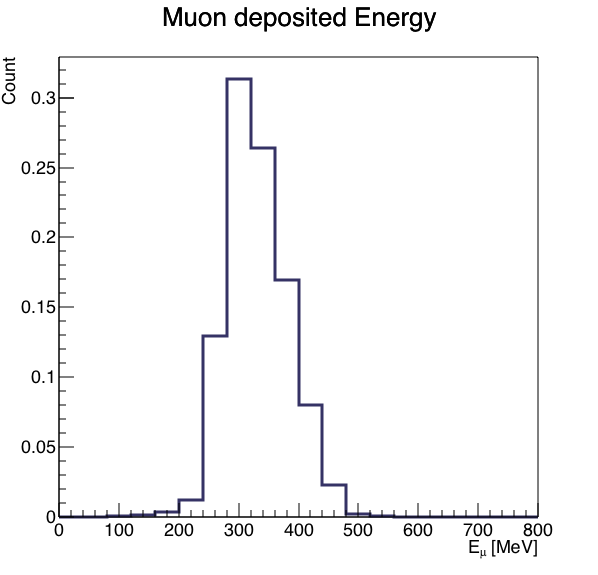
\includegraphics[width=3in]{pMuGamma/MuonMCEn.png}
\caption{Deposited energy distribution of the muon at MCReco level. All cuts in Table \label{T3} have been applied. The plot is area normalized. }
\label{F1}
\end{minipage}\hfill
\begin{minipage}{0.45\textwidth}
\centering
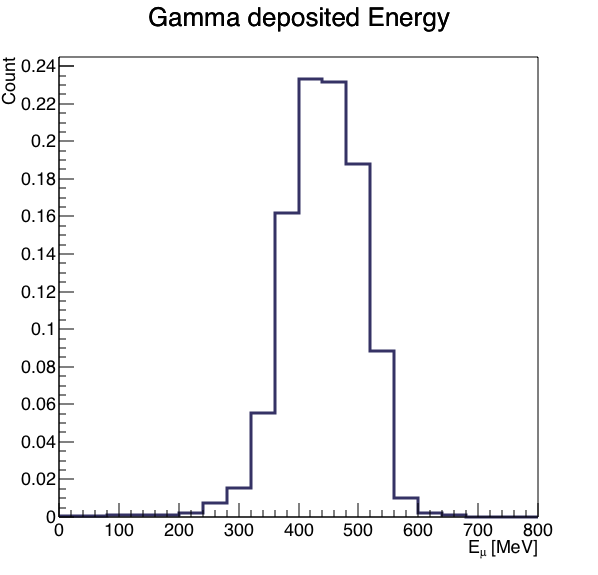
\includegraphics[width=3in]{pMuGamma/GammaMCEn.png}
\caption{Deposited energy distribution of the gamma at MCReco level. All cuts in Table \label{T3} have been applied. The plot is area normalized.}
\label{F2}
\end{minipage}
\end{figure}



\begin{figure}[htbp]
\begin{center}
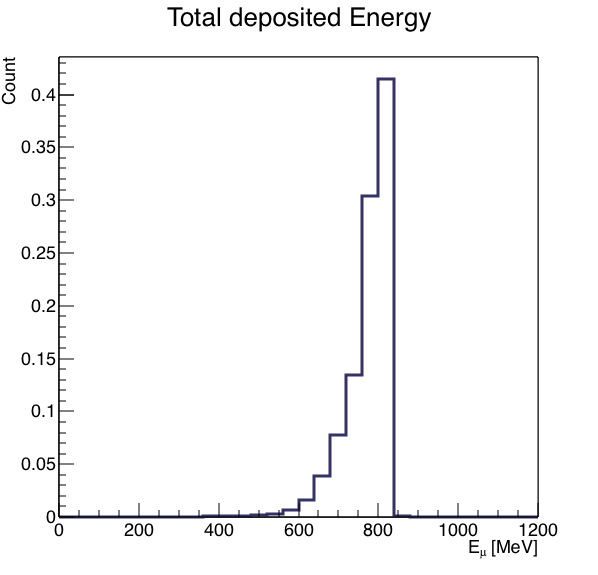
\includegraphics[width=4in]{pMuGamma/ProtonMCEn.png}
\caption{Candidate deposited energy at MCReco level. All cuts in Table \label{T3} have been applied. The plot is area normalized.}
\label{F3}
\end{center}
\end{figure}


\begin{figure}[phbt]
\centering
\begin{minipage}{0.45\textwidth}
\centering
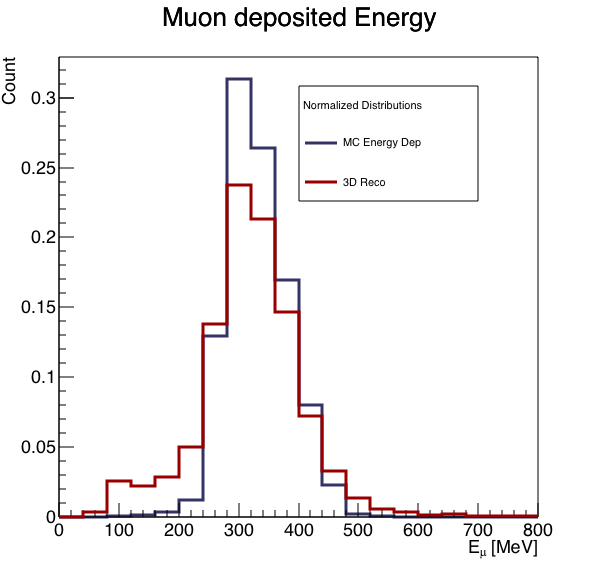
\includegraphics[width=3in]{pMuGamma/MuonSame.png}
\caption{Deposited energy  of the  muon at MCReco and Reco level. All cuts in Table \ref{T3} have been applied. The two plots are area normalized.}
\label{F4}
\end{minipage}\hfill
\begin{minipage}{0.45\textwidth}
\centering
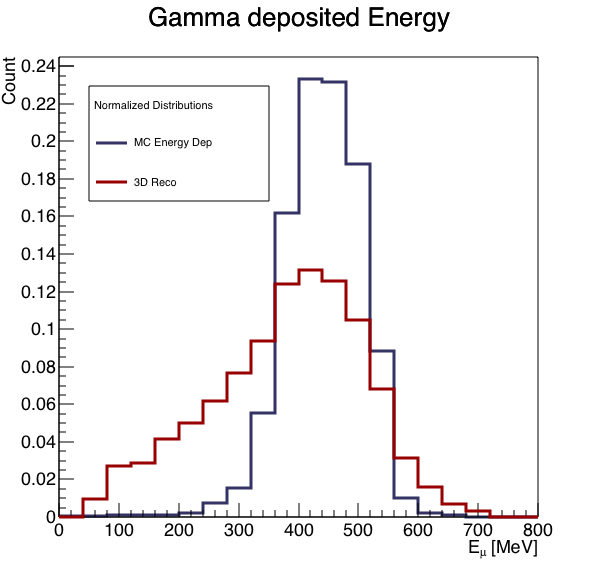
\includegraphics[width=3in]{pMuGamma/GammaSame.png}
\caption{Deposited energy  of the  gamma at MCReco and Reco level. All cuts in Table \ref{T3} have been applied. The two plots are area normalized.}
\label{F5}
\end{minipage}
\end{figure}



\begin{figure}[hpbt]
\centering
\begin{minipage}{0.45\textwidth}
\centering
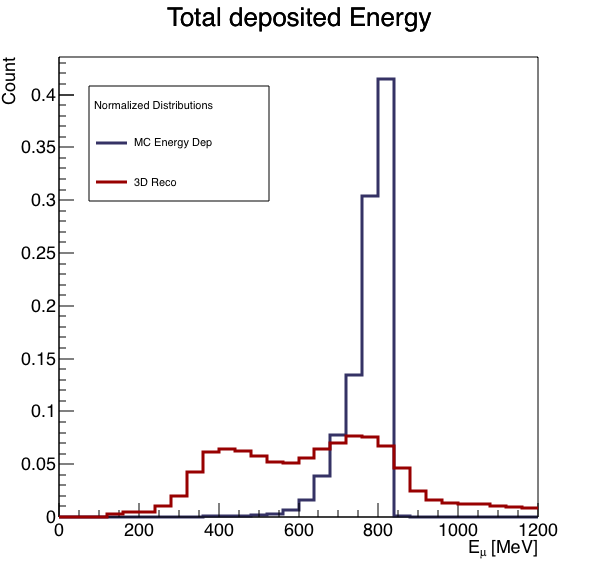
\includegraphics[width=3in]{pMuGamma/ProtonSameNoCut.png}
\caption{Candidate deposited energy at MCReco and Reco level. No cuts in Table \ref{T3} have been applied for Reco. The two plots are area normalized.}
\label{F6}
\end{minipage}\hfill
\begin{minipage}{0.45\textwidth}
\centering
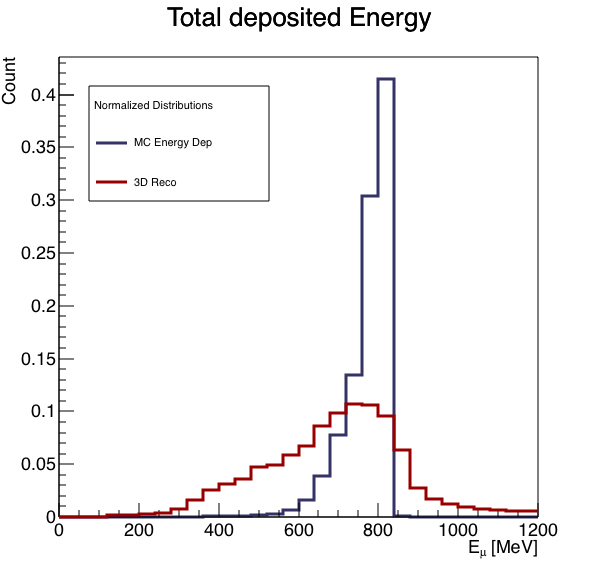
\includegraphics[width=3in]{pMuGamma/ProtonSameGeo.png}
\caption{Candidate deposited energy at MCReco and Reco level. Only geometrical cuts in Table \ref{T3} have been applied for Reco. The two plots are area normalized.}
\label{F7}
\end{minipage}\hfill
\begin{minipage}{0.45\textwidth}
\centering
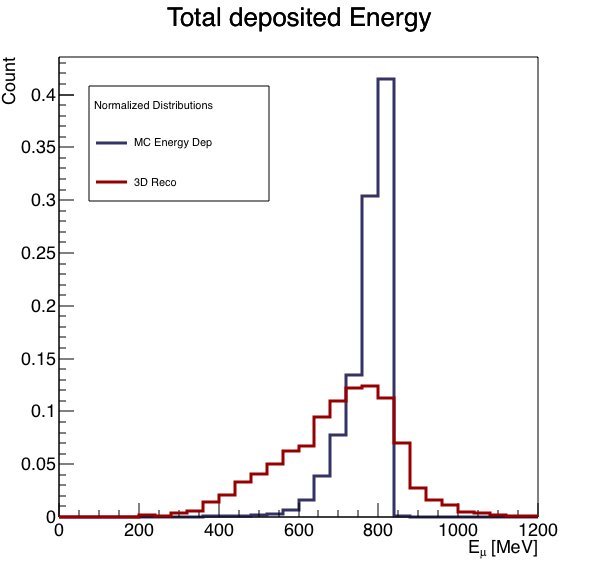
\includegraphics[width=3in]{pMuGamma/ProtonSameGeoAndEn.png}
\caption{Candidate deposited energy at MCReco and Reco level. All cuts in Table \ref{T3} have been applied for Reco. The two plots are area normalized.}
\label{F8}
\end{minipage}
\end{figure}

\clearpage
\section{$p \rightarrow e^{+} \pi^{0}$}
The following paragraphs address the analysis of the  $e^{+} \pi^{0}$ proton decay mode, a dominant decay mode in many GUT models. This is the ``golden mode" for water Chrenkov detectors and will serve as a standard candle.\\
The neutral pion decays immediately into two photons, both of which produce EM showers in the detector. The positron showers as well, leading to a signal topology of three electromagnetic showers emerging from a common origin.

The aim of what follows is to describe a set of cuts designed to isolate this signal from background, and to further discuss the types of cosmogenic background events that can fake this signal.

\subsection{Signal only analysis}

In an attempt to isolate this signal, the following procedure was implemented (for a detailed explanation about running the code, see Appendix A ):
\begin{enumerate}[topsep=10pt,itemsep=-1ex,partopsep=10pt,parsep=1ex]
\item Shower filter
\item Strict $e^{+}$ identification
\item Strict $\pi^{0}$ identification
\item Loose $e^{+}$ identification
\item Loose $\pi^{0}$ identification
\item Geometrical cuts
\item Calorimetric cuts
\end{enumerate}


\subsubsection{Shower filter}

The first stage of event selection is the shower filter. A three shower filter is imposed that discards all events without three reconstructed showers. Though in future analyses, this will be changed to reject all events with fewer than three reconstructed showers, it was beneficial for a preliminary step of this analysis to impose a strict three shower cut on signal sample because it allows for the identification efficiency of this event topology to be partially separated from shower reconstruction efficiencies. This analysis depends crucially on accurate shower reconstruction, which is still under development. By limiting the analysis to signal events that have exactly three reconstructed showers, there is a greater likelihood that the showers have been reconstructed reasonably well. Even so, shower reconstruction effects still dominate the factors contributing to the loss of signal events.

\subsubsection{Particle identification}

After the shower filter, a first attempt at particle identification is performed. The strategy for particle identification is to loop through reconstructed showers and to try to associate the shower with either a positron or photon from neutral pion decay. It is superior at this stage to over-identify pions and positrons in the event because further cuts are applied later to eliminate misreconstructed particles. If the identification is too tight, there is a risk of losing good events at this stage. Since the identification is performed sequentially, however, only one loose pass cannot be performed because the first identification algorithm applied will misidentify certain showers as its own. For concreteness, take the example of searching for a neutral pion  first, using a loose definition. This algorithm may reconstruct pions using the shower actually coming from the positron, eliminating it from the viable pool of showers when the positron identification algorithm is applied next.

To circumvent this, particle identification is performed iteratively. First, positrons and neutral pions are identified according to a tight definition so that only showers that are very likely to be correctly associated with that particular particle are associated with it. Then, a looser iteration is performed on the remaining showers. This methodology helps to avoid the problem of ``overzealous identification" for a particular particle.

Both the tight and loose definitions employed for particle identification are displayed in Tables \ref{t1} and \ref{t2}. The $e$-like nature of a shower is found by comparing the log-likelihood of its $dE/dx$ corresponding to a photon or electron as described in sec \ref{ID}. 

The definition of ``likelihood" for the neutral pion is similar but takes into consideration five different aspects of the reconstruction. The likelihood is the sum of the log-likelihoods of the radiation length for both $\gamma$ showers, the $dE/dx$ for both showers, and the impact parameter for the two showers. The log-likelihoods are defined identically to the definitions supplied above but different PDFs are used for radiation length and impact parameter.

It should be noted that a particularly strong discriminating variable in $\pi^{0}$ identification is the angle between the two $\gamma$ showers. For a given $\pi^{0}$ energy, there is a fixed minimum angle between the showers $\alpha_{\text{min}} = 2\arcsin(\frac{m_{\pi}}{E_{\pi}}) = 2\arcsin(1/\gamma)$. This can be calculated by boosting a back-to-back decay from the rest frame of the pion into a frame moving perpendicularly to the photons. As can be seen in Figure 4, the distribution of $\theta_{\gamma\gamma}$ drops sharply to zero below the minimum angle for this energy range, roughly 0.45 radians. This provides a good handle on identifying pions in the appropriate energy range.

\begin{table}[!hbtp]
\centering
\caption{Cuts applied during $e^{+}$ identification for both loose and tight IDs.}
\begin{tabular}{|l|l|l|}
\hline
\multicolumn{1}{|c|}{{\bf Parameter}} & {\bf Tight Cut}  & {\bf Loose Cut}  \\ \hline
$dE/dx$                               & is $e$-like 	 & is $e$-like \\ \hline
Shower energy                         & $> 200$ MeV      & $> 100$ MeV      \\ \hline
\end{tabular}
\label{t1}
\end{table}

\begin{table}[!hbtp]
\centering
\caption{Cuts applied during pion identification for both loose and tight IDs.}
\begin{tabular}{|l|l|l|}
\hline
\multicolumn{1}{|c|}{{\bf Parameter}} & {\bf Tight Cut}         & {\bf Loose Cut}         \\ \hline
``Likelihood"                         & $> -10$                 & $> -10 $       		  \\ \hline
IP of two showers                     & $< 5$ cm          		& $< 10$ cm		         \\ \hline
Pion mass                             & {[}100, 200{]} MeV      & {[}75, 275{]} MeV       \\ \hline
Shower energies                       & {[}20, 600{]} MeV       & {[}15, 1000{]} MeV      \\ \hline
Angle between showers                 & {[}0.5, 3.14{]} radians & {[}0.3, 3.14{]} radians \\ \hline
Pion energy                           & $> 100$ MeV             & $> 100$ MeV             \\ \hline
\end{tabular}
\label{t2}
\end{table}

\subsubsection{Geometrical cuts}

After particle identification has been performed, two geometrical cuts are applied to try to identify the topology of proton decay. The first is a cut on the radius of the smallest sphere that encloses the start points of the three showers. This serves as a proximity cut. This radius is a more robust variable to cut on than the distance between the reconstructed $\pi^{0}$ location and the start point of the positron shower. This is because during pion reconstruction, the position of the neutral pion is determined by finding the point of closest approach between the two half-lines extending from the photon showers in the opposite direction from the reconstructed shower direction. If the shower direction is even slightly misreconstructed, the change in angle can change the point of closest approach significantly. For this reason, using the reconstructed pion position as a parameter to cut on is inadvisable. In contrast, the positions of the initial energy deposits for the showers is a quantity measured directly by the detector and is therefore subject to less uncertainty due to reconstruction effects.
%The radiation length of the photon is on the order of 30 cm (MAYBE?? need citation) but SOME PHOTONS TAKE FOREVER SO BIG CUT BIG CUT INCLUSIVE YEAH

The second geometrical cut performed is a cut on the angle between the 3-momenta of the reconstructed $\pi^{0}$ and $e^{+}$. Naively, this would be expected to be steeply peaked near $\pi$ because the proton decays at rest and momentum is conserved. This is not the case. Two factors contribute to this. The first is that the proton does not decay at rest, but instead decays with some momentum less than the Fermi momentum of the nucleus, which is on the order of 215 MeV/$c$.  In addition to this effect, the angle between the decay products is changed because the pion undergoes intranuclear interactions before escaping the nucleus that can alter its momentum. For these reasons, the cut on angle is very loose.


\subsubsection{Calorimetric cuts}

After geometrical cuts are performed, calorimetric cuts on the decay products and reconstructed proton are performed. These consist of a simple energy cut on the reconstructed positron and pion as well as an energy cut on the reconstructed proton (found by summing the four-momenta of the electron and pion). The energy of the positron is taken to the be the total energy associated with the shower. The energy of the $\pi^{0}$ is found by reconstructing the momentum and invariant mass of the $\pi^{0}$ according to the following two equations:
\begin{equation}
|P_{\pi^{0}}| = \sqrt{E_1^2 + E_2^2 + 2E_1 E_2 \cos(\theta_{\gamma\gamma})}
\end{equation}
and
\begin{equation}
M_{\gamma\gamma} = \sqrt{4E_1^{\gamma} E_2^{\gamma} \sin^2 (\theta_{\gamma\gamma} / 2)}
\end{equation}
where $E_1$ and $E_2$ are the energies of the $\gamma$ showers and $\theta_{\gamma\gamma}$ is the opening angle between the showers~\cite{Acciarri:2014isz}. Note that substituting these formulas into $E^2 = p^2 c^2 + m^2 c^4$ returns $E_{\pi^{0}} = E_1 + E_2$, the sum of the energy depositions of the two photons.

Additionally, cuts are applied on the components of the reconstructed proton 3-momentum to seek out decays in which the proton has initial momentum not much larger than the Fermi momentum.

\subsection{Results}

The preliminary results presented below show the efficiency of this selection methodology at the MCReco and Reco level. 
%The first is ``truth level," which corresponds to truth information at generator level. The second is ``Monte Carlo energy deposition," terms used to describe the information about energy depositions in the detector that are associated with truth particles. Thirdly, there is reconstruction, which consists only of the information reconstructed from measured quantities in the detector.

Table \ref{t3} shows that the cutflow keeps a good percentage of events when applied to MCReco level. This is not true at the reconstruction level. The cause of such a low efficiency seems to be due primarily to shower reconstruction effects. For example, two-thirds of events are lost because the number of reconstructed showers is not equal to 3. On top of this, $\pi^{0}$ reconstruction is poor at reco level and requires further work. The overall efficiency for this channel is $\sim$ 2\%.

\begin{table}[!htbp]
\centering
\caption{Topology-based and calorimetry-based set of cuts to identify proton decay. All samples are signal only. The poor efficiency of the reconstructed events is due predominately to shower reconstruction effects.}
\begin{centering}
\begin{tabular}{|l|l|l|l|}
\hline
\multicolumn{1}{|c|}{{\bf Parameter}}    & {\bf Cut}      & {\bf MCReco} & {\bf Reco} \\ \hline
Initial total                            & -                  & 9990                      & 9960       \\ \hline
Shower filter                            & 3 showers in event         & 9867               & 3222       \\ \hline
IDed $\pi^0$s in event                   & $> 1$                     & 9551               & 1753       \\ \hline
IDed $e^{+/-}$s in event                 & $> 1$                     & 9548               & 932        \\ \hline
Radius of sphere enclosing shower starts & $< 50$ cm                  & 9373               & 546        \\ \hline
Angle between $e^+$ and $\pi^0$          & $> 2$ radian              & 9337               & 396        \\ \hline
$e^+$ energy                             & $> 200$ MeV              & 9334               & 381        \\ \hline
$\pi^0$ energy                           & $> 250$ MeV               & 9324               & 347       \\ \hline
Proton energy                            & {[}800, 1000{]} MeV         & 9164               & 223         \\ \hline
$|\Sigma p_x|$, $|\Sigma p_y|$, $|\Sigma p_z|$ & $< 300$ MeV                & 9039               & 190         \\ \hline
\end{tabular}
\end{centering}
\label{t3}
\end{table}



Despite the low efficiency, the events that are selected as proton decay candidates at reco level do seem to be well-reconstructed events, indicating that the selection behaves well. Figures \ref{figure1} and \ref{f2} demonstrate this. Figure \ref{figure1}  shows the positron energy at both the levels of analysis after all cuts have been applied. From MC energy deposition to reco, the distribution broadens slightly due to imperfections in clustering and shower reconstruction. Despite this, the peak appears to be in roughly the same position and the distributions are comparably shaped, indicating that the events selected, though few, were well-reconstructed. Therefore, for well-reconstructed events, our selection appears to work well to identify the three shower topologies associated with this channel of proton decay.


Figure  \ref{f2} shows the same plot for the $\pi^{0}$ energy. Here, the distribution has been shifted significantly downward. This is due mainly to reconstruction inefficiencies. It is interesting to notice that the reconstruction of the boosted $\pi^{0}$ is particularly difficult due to the high collimation of the decay products leading to overlapping showers. The primary error made during the reconstruction of these events is to reconstruct the $\pi^{0}$ as a single, highly-energetic shower.  In fact, 4360 signal events out of 9960 total have two reconstructed showers or fewer. By hand-scanning a small portion of them, we noticed that the overlapping showers tend to be reconstructed as some set of showers and tracks. In three shower events specifically, the energy of the $\pi^{0}$ is lower because some of the particle's energy has been reconstructed as tracks. A strategy to improve these reconstruction efficiencies may be to extend the $\pi^{0}$ algorithm by searching for reconstructed showers with $dE/dx \approx 8.5$ MeV/$c^2$ that correspond to the combination of two $\gamma$-showers. This methodology would also allow for the identification of Dalitz decay, a decay mode of $\pi^{0}$ to which this analysis is currently not sensitive.


Figure \ref{f3} shows the energy of the reconstructed proton (sum of decay product 4-momenta) at each level. Though there is significant variation in the distribution, it appears to peak slightly below the truth energy, an effect that is the result of the misreconstruction of the pion energy discussed previously.

\begin{figure}[p]
\begin{center}
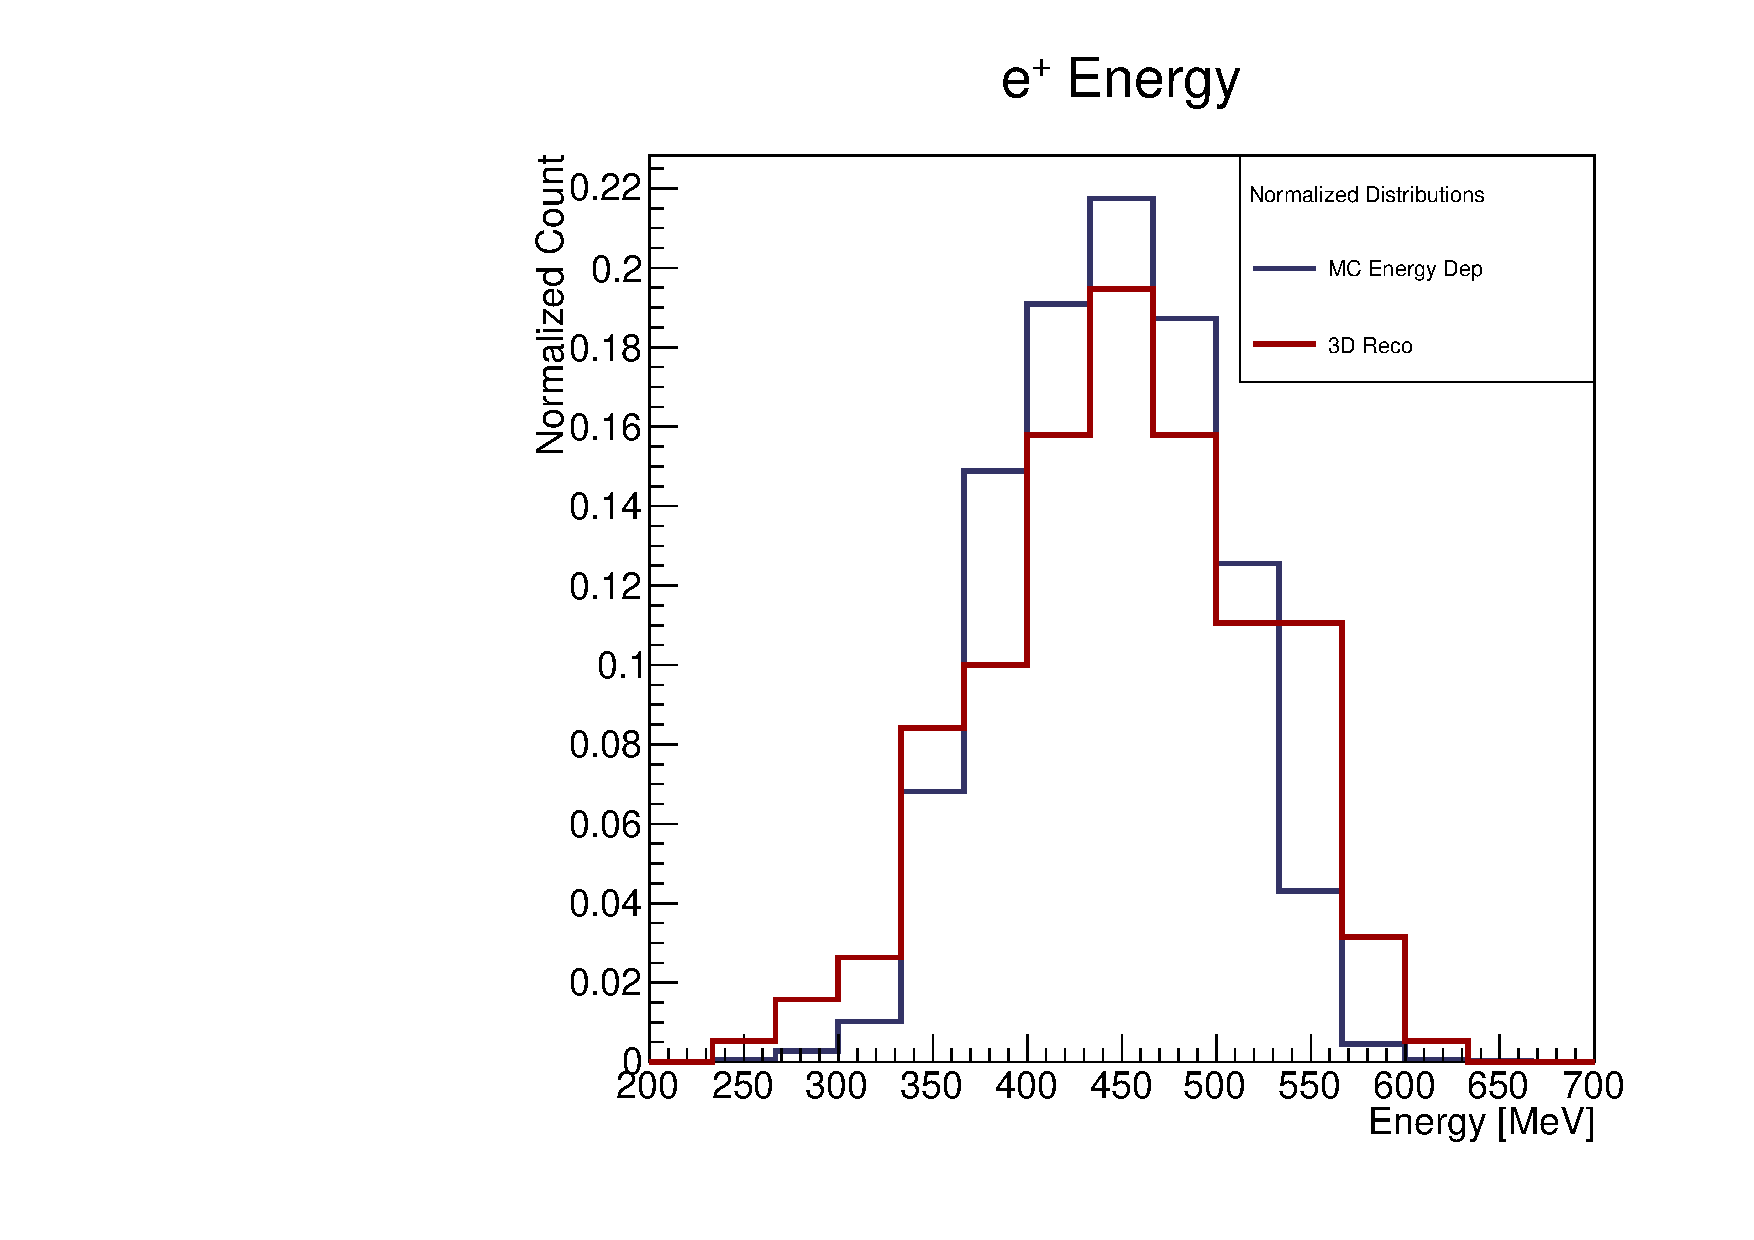
\includegraphics[width=4in]{pPi0E/e_eplus_postcutcomp.pdf}
\caption{Energy distributions of the  positron at MCReco and Reco level. All cuts in Table \label{t3} have been applied. The two plots are area normalized.}
\label{figure1}
\end{center}
\end{figure}

\begin{figure}[htb]
\begin{center}
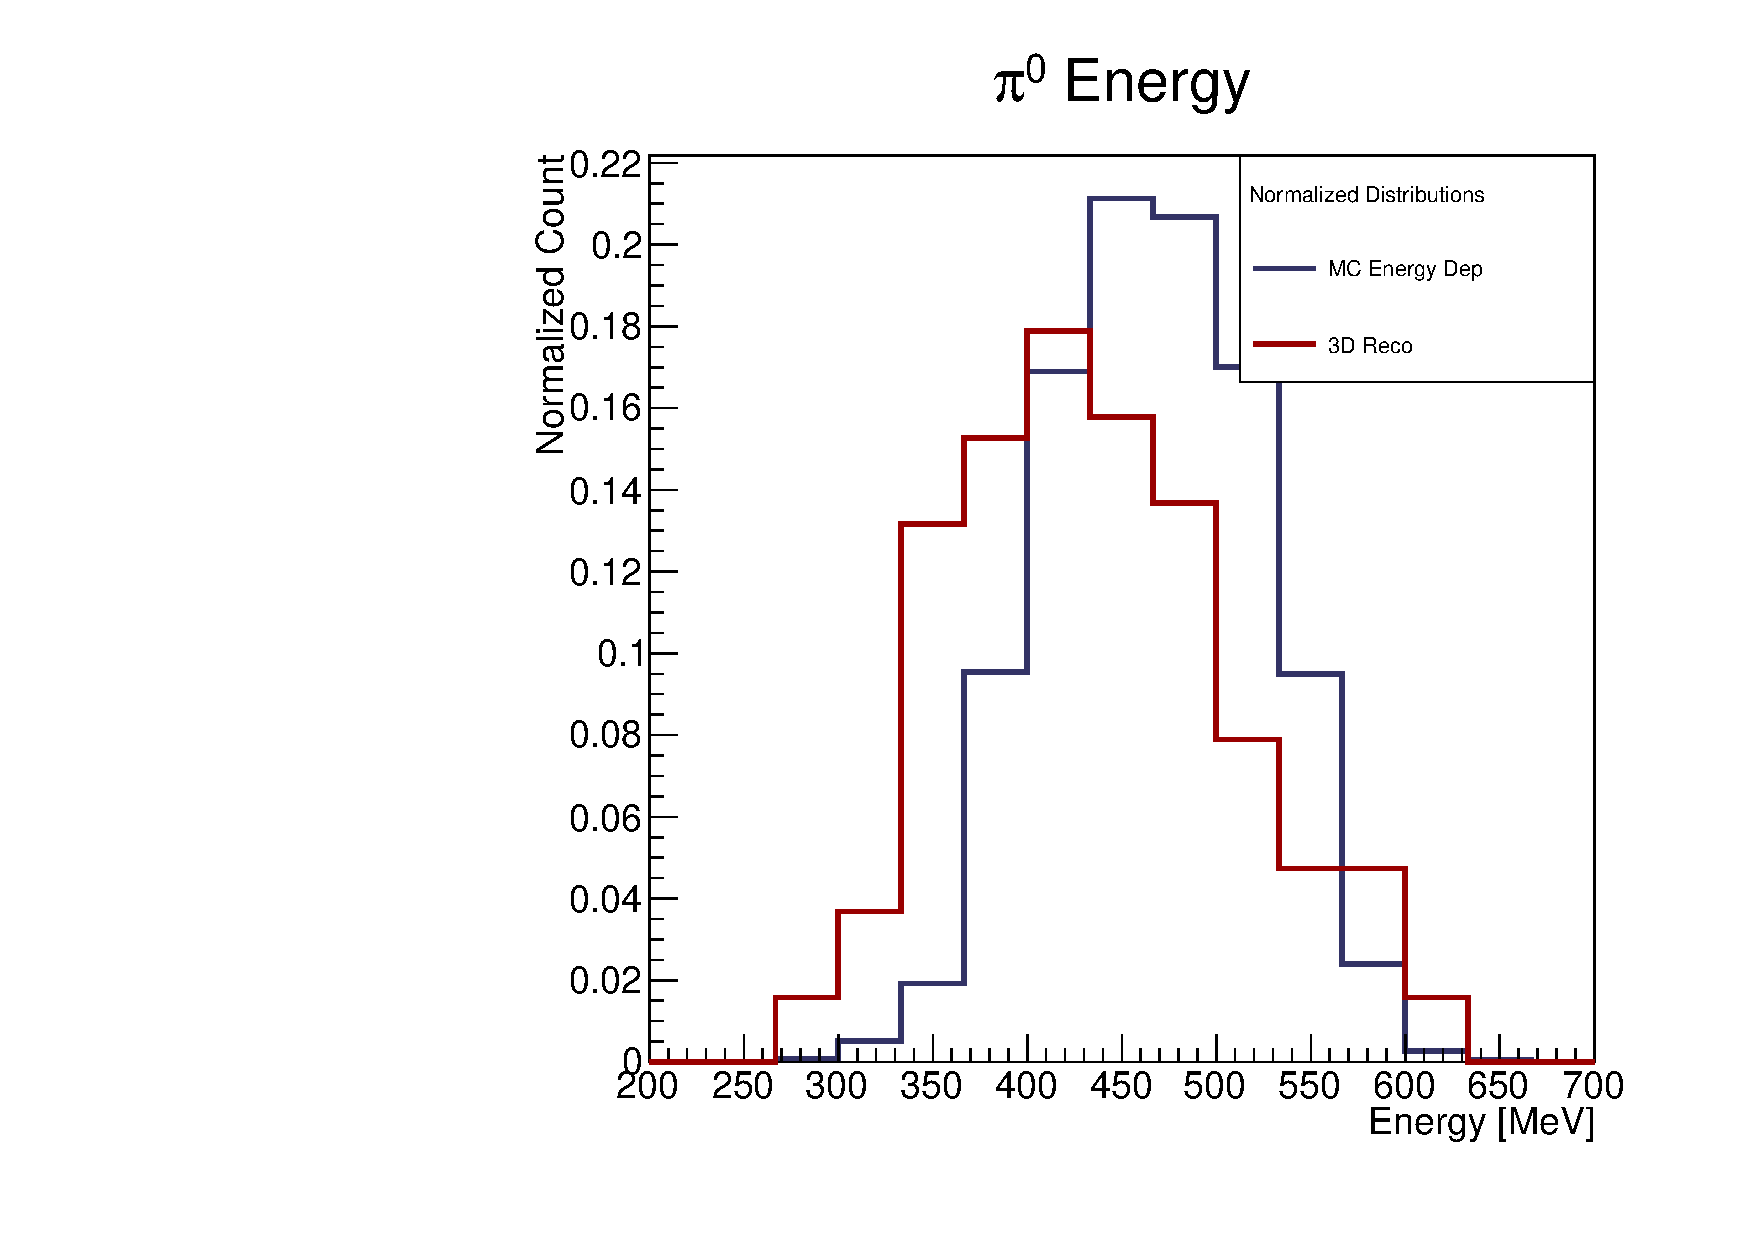
\includegraphics[width=4in]{pPi0E/e_pion_postcutcomp.pdf}
\caption{Energy distributions of the pion at MCReco and Reco level. All cuts in Table \label{t3} have been applied. The two plots are area normalized.}
\label{f2}
\end{center}
\end{figure}

\begin{figure}[htbp]
\begin{center}
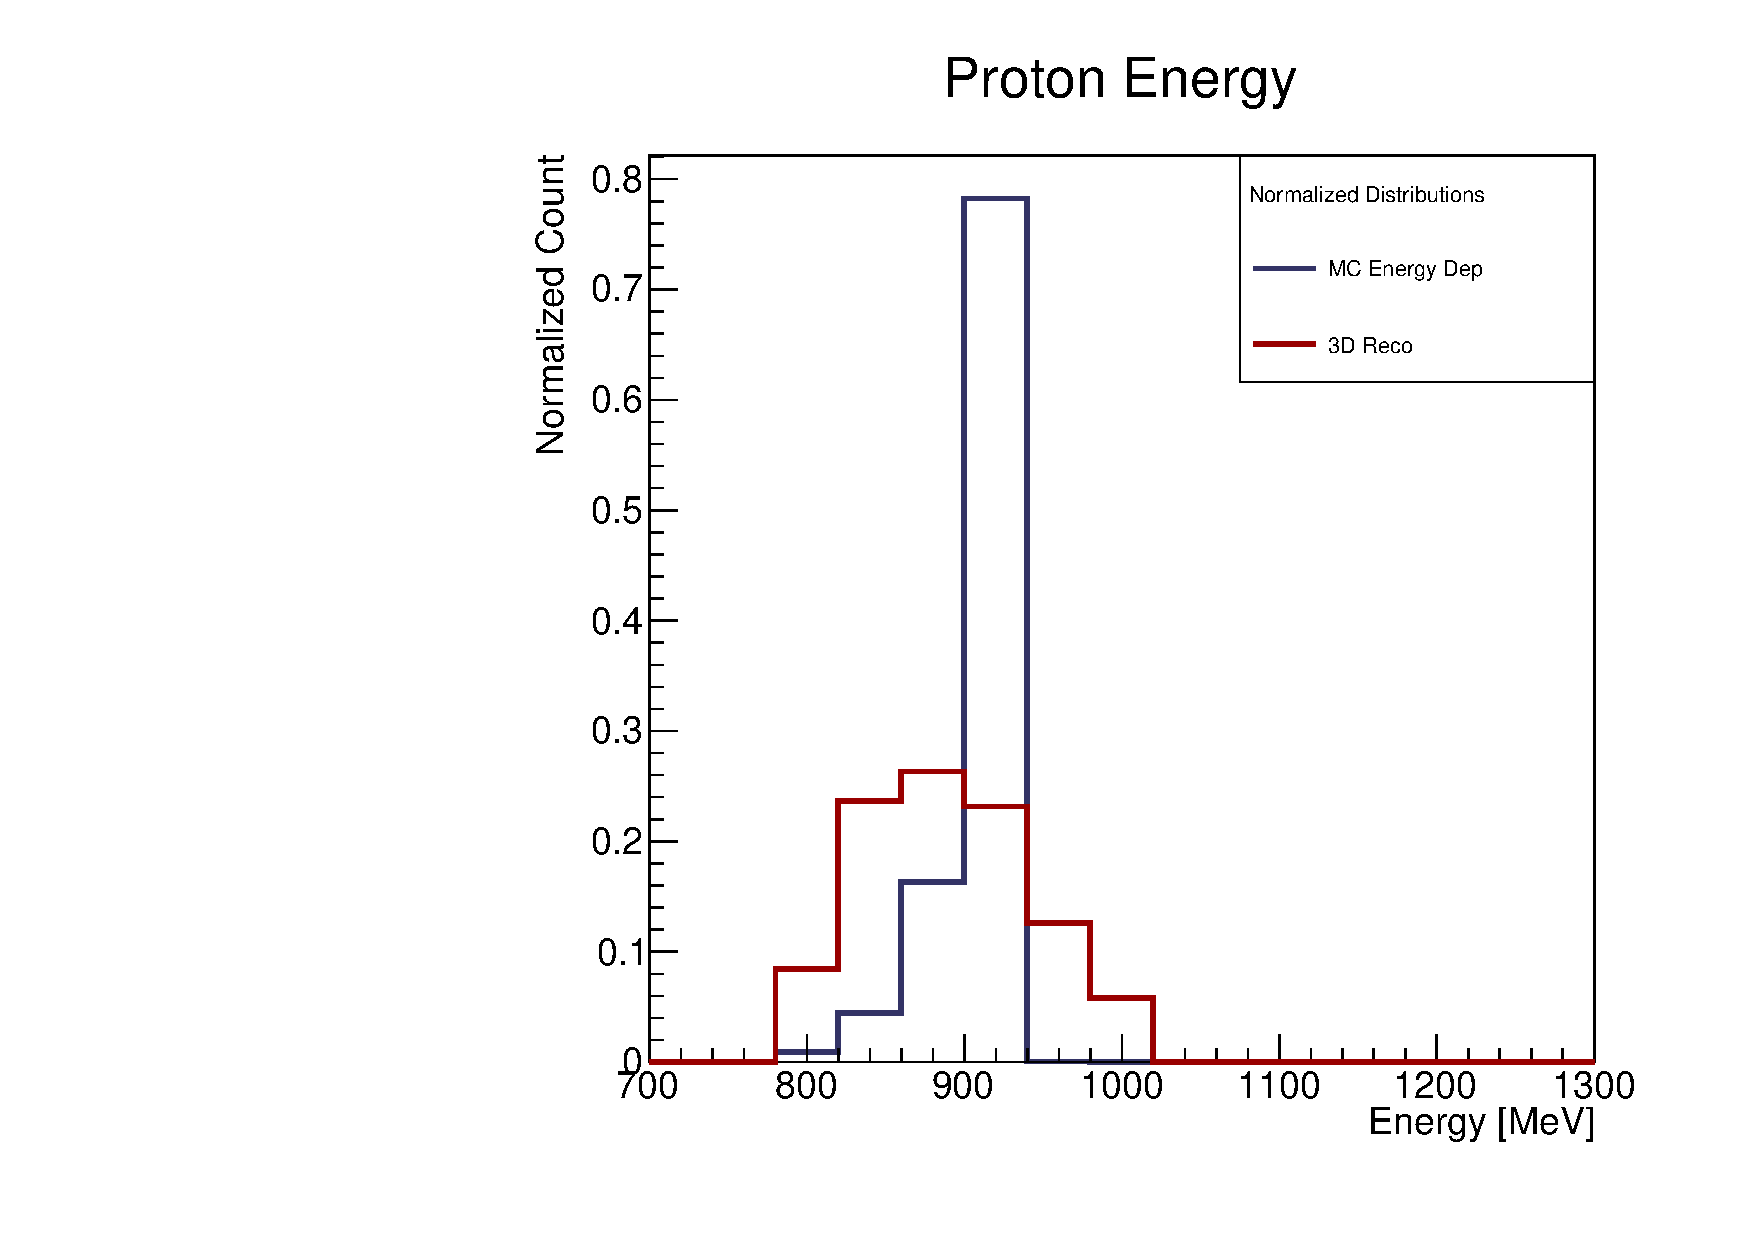
\includegraphics[width=4in]{pPi0E/e_proton_postcutcomp.pdf}
\caption{Energy distributions of the reconstructed proton at MCReco and Reco level. All cuts in Table \label{t3} have been applied. The two plots are area normalized.}
\label{f3}
\end{center}
\end{figure}



%If, in the clustering stage of reconstruction, some part of a shower is missed, the angle can be skewed. As discussed previously, a small angular uncertainty can become a large uncertainty on other quantities, including the invariant mass. This can be seen in Figure 4, which plots the invariant mass of the pion at all three stages. Ideally, it would be a $\delta$-function at the true value of the $\pi^{0}$ mass (135 MeV/$c^2$), but the invariant mass is very broadly distributed at reco level due to errors in reconstruction.

%Though the distribution is shifted, it is still roughly comparable to the truth distribution. Compare this with Figure 4, which shows these distributions for all selected pions before any cuts beyond those imposed in Table 2 are applied. The distribution.

\section{Conclusions}

%The results of this preliminary investigation indicate that there is the potential to have a high selection efficiency for $p \rightarrow \mu^{+} \gamma$  and $p \rightarrow e^{+} \pi^{0}$ in MicroBooNE and other LArTPCs. These results can only improve as reconstruction in MicroBooNE improves.

\nocite{*}
\bibliographystyle{unsrt}
\bibliography{bib}


\appendix

\section{Manual}

This section will explain the machinery used to perform this analysis. The modules for topology identification were all written within ERTool, a lightweight analysis framework for Larlite data products. This assumes that you already have LArLite installed and compiled.\\

All of the modules used for this are stored in the ``Ndk" git repository. To clone this, run\\

\texttt{git clone git@github.com:ElenaGramellini/Ndk.git} \\

\noindent
For $p \rightarrow e^{+} \pi^{0}$ , 

\texttt{cd Mode0}

\noindent
and

\texttt{make}.

Within the directory, there are multiple modules that are run during the analysis, primarily\\
 \texttt{ShowerFilter\_NdkModeZero.cxx}, \texttt{ERAlgoSingleE\_NdkModeZero.cxx}, \texttt{ERAlgoPi0\_NdkModeZero.cxx}, \\ and \texttt{ERAnaNdkModeZero.cxx}. \\
Unless you need to fix a bug, there should be no need to interact directly with these modules once they are compiled. Everything is done instead through the launcher macro \texttt{modezeroselection.py}, located under \texttt{mac/}.

To run this, use

\texttt{python mac/modezeroselection.py [\textit{filename}] $>$ log.log \&}.

\noindent
This will run the analysis over \textit{filename} (a LArLite file) in the background and redirect \texttt{stdout} to \texttt{log.log} so you can read the status using \texttt{tail -f log.log}. Running this will output a ROOT file that contains several plots and a TTree containing the information about all the identified pions and electrons in the sample provided.

There are various parts of \texttt{modezeroselection.py} that must be changed each time a new sample is analyzed. First, there is the output filename (line 21). Change the name after \texttt{outfile = } to be whatever output file you want. If you plan on running over an MCTruth file, you must set \texttt{mc} to \texttt{True}, otherwise, \texttt{False} (line 18). Lines 29 and 30 let you set the minimum and maximum number of showers accepted in a given event.

Lines 36-72 allow you to modify the cuts placed when identifying $\pi^{0}$s and $e^+$s. Most are self-explanatory. For the electrons, there is only one that matters (\texttt{setEThreshold}, which sets the energy value that any candidate electron must be above). The others are deprecated. For the pion, you can specify minimum and maximum shower energy, maximum impact parameter between the two showers, minimum and maximum reconstructed mass, and minimum and maximum angle between the two showers.

Once this step has been completed, the actual cutflow can be applied to the reconstructed pions and electrons stored in \texttt{outfile}. To do this, we use another macro, \texttt{mac/ModeZero\_cutflow\_v3.py}.

To run, do

\texttt{python mac/ModeZero\_cutflow\_v3.py [\textit{outfile}]}

\noindent
where \textit{outfile} refers to the ROOT file output at the end of the previous step. This will return a new ROOT file with histograms of relevant quantities. The actual yield will be output to \texttt{stdout} when the process finishes.

There are also many tunable parameters at this stage. They can be found in lines 11-35. The first thing to note is the ability to specify the output filename (edit \texttt{cutflowoutputfile =}). Then, there is the \texttt{doTruth} option, which must be \texttt{False} for any reco files and can be either \texttt{True} or \texttt{False} for MCTruth files (this will access the truth branches of the TTree and so will throw an error if there are no truth branches). Then there are the parameters, each of which has an associated comment describing the cut.

The files used for this study (at the time of writing) are as follows:
\begin{enumerate}[topsep=10pt,itemsep=-1ex,partopsep=10pt,parsep=1ex]
\item Truth signal: \url{/pnfs/uboone/scratch/users/elenag/v04_12_00/Mode0/sim/prod_NdK/2597833_*/larlite_mcinfo_*.root}
\item Reco signal: \url{/pnfs/uboone/scratch/users/elenag/v04_12_00/Mode0/reco2/prod_NdK/*_*/larlite_reco3d.root}
\end{enumerate}

\section{$e^{-}$ vs. $\gamma$ Particle Identification}
Given a reconstructed electromagnetic (EM) shower, a particle type is assigned as $e^{-}$ or $\gamma$ using
a log-likelihood ratio ($\mathcal{LL}$) method. This appendix describes about both a procedure and algorithm source code repository.

\subsection{Procedure}
There are two probability density functions (PDFs) defined and used for likelihood calculation: one
is for a particle's radiation length [cm], and the other for dE/dX [MeV/cm]. The former is a simple
exponential function while the latter is a simple gaussian for electron and double-gaussian for gamma.
A reason for using double-gaussian for gamma's dE/dX is to account for a small peak at 2 MeV/cm for gamma
showers with a mis-reconstructed start point.
\begin{eqnarray}
  \text{Radiation Length PDF}_{e^{-}/\gamma} &=& \exp\left(-x/\mathcal{L}_{rad.}\right)\\
  \text{dE/dx PDF}_{e^{-}} &=& \exp\left(-\frac{(x-\mu)^2}{2\sigma^2}\right)\\
  \text{dE/dx PDF}_{\gamma} &=& \exp\left(-\frac{(x-\mu_1)^2}{2\sigma_1^2}\right) + N\times\exp\left(-\frac{(x-\mu_2)^2}{2\sigma_2^2}\right)
\end{eqnarray}
\begin{figure}[htb]
\begin{center}
  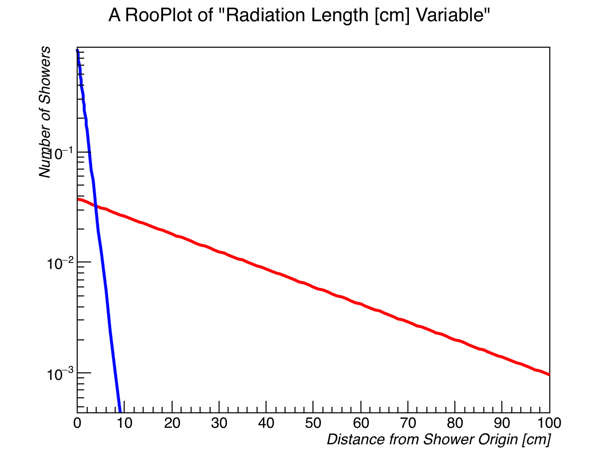
\includegraphics[width=3in]{RadLength.png}
  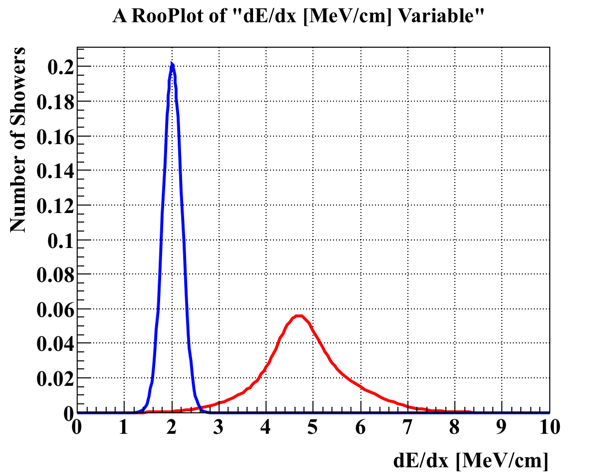
\includegraphics[width=3in]{dEdx.png}
  \caption{Probability density function of a radiation length [cm] (left) and dE/dx [MeV/cm]
    for electron (blue) and gamma ray (red). Values are tuned using MCReco information from single
    $e^{-}$ and $\gamma$ MC samples.}
  \ref{fig:algoempart}
\end{center}
\end{figure}
The default parameter set for these PDFs are tuned using MCReco showers from single $e^{-}$ and $\gamma$
MC sample with an artificially widened width which comes from a resolution from reconstructed shower.
This is shown in Fig.\ref{fig:algoempart}.

Then electron/gamma likelihood is defined as
\begin{eqnarray}
  \mathcal{LL}_{e^-}\left(dE/dx,\mathcal{L}_{rad}\right) &=& \frac{\text{PDF}_{e^-}(dE/dx,\mathcal{L}_{rad})}{\text{PDF}_{e^-}(dE/dx,\mathcal{L}_{rad}) + \text{PDF}_{\gamma}(dE/dx,\mathcal{L}_{rad})}\\
    \mathcal{LL}_{\gamma}\left(dE/dx,\mathcal{L}_{rad}\right) &=& \frac{\text{PDF}_{\gamma}(dE/dx,\mathcal{L}_{rad})}{\text{PDF}_{e^-}(dE/dx,\mathcal{L}_{rad}) + \text{PDF}_{\gamma}(dE/dx,\mathcal{L}_{rad})}
\end{eqnarray}
and a particle type of each EM shower is assigned based on above formula with higher return value.

\subsection{Toolkit}
The procedure described above is implemented in a {\ttfamily C++} toolkit {\ttfamily ERTool}.
In particular {\ttfamily ertool::AlgoEMPart} is responsible for this $e^-$ vs. $\gamma$ separation
method in {\ttfamily ertool::AlgoEMPart::LL} function. One can find a source code at
\begin{lstlisting}
$LARLITE_USERDEVDIR/SelectionTool/ERTool/Algo/AlgoEMPart.h
\end{lstlisting}
Underlying fitting framework is {\ttfamily RooFit} which comes as a standard extension of {\ttfamily ROOT}
software framework. PDFs are implemented as an extension of {\ttfamily RooFit} PDF classes in the following
source code.
\begin{lstlisting}
$LARLITE_USERDEVDIR/SelectionTool/ERTool/Base/PdfFactory.h
\end{lstlisting}


\end{document}
